\documentclass[11pt]{diazessay} % Font size (can be 10pt, 11pt or 12pt)

%----------------------------------------------------------------------------------------
%	TITLE SECTION
%----------------------------------------------------------------------------------------

\title{\textbf{Relations Between Topological Spaces} } % Title and subtitle

\author{Liguang Hou} % Author and institution

\date{\today} % Date, use \date{} for no date

%----------------------------------------------------------------------------------------

\begin{document}
\maketitle % Print the title section

%----------------------------------------------------------------------------------------
%	ABSTRACT AND KEYWORDS
%----------------------------------------------------------------------------------------

%\renewcommand{\abstractname}{Summary} % Uncomment to change the name of the abstract to something else

\begin{abstract}

	\noindent
	This paper summarized some basic topological spaces and their relationships as below.
	
	\vskip 5pt
	\begin{figure}[h]
		\centering
		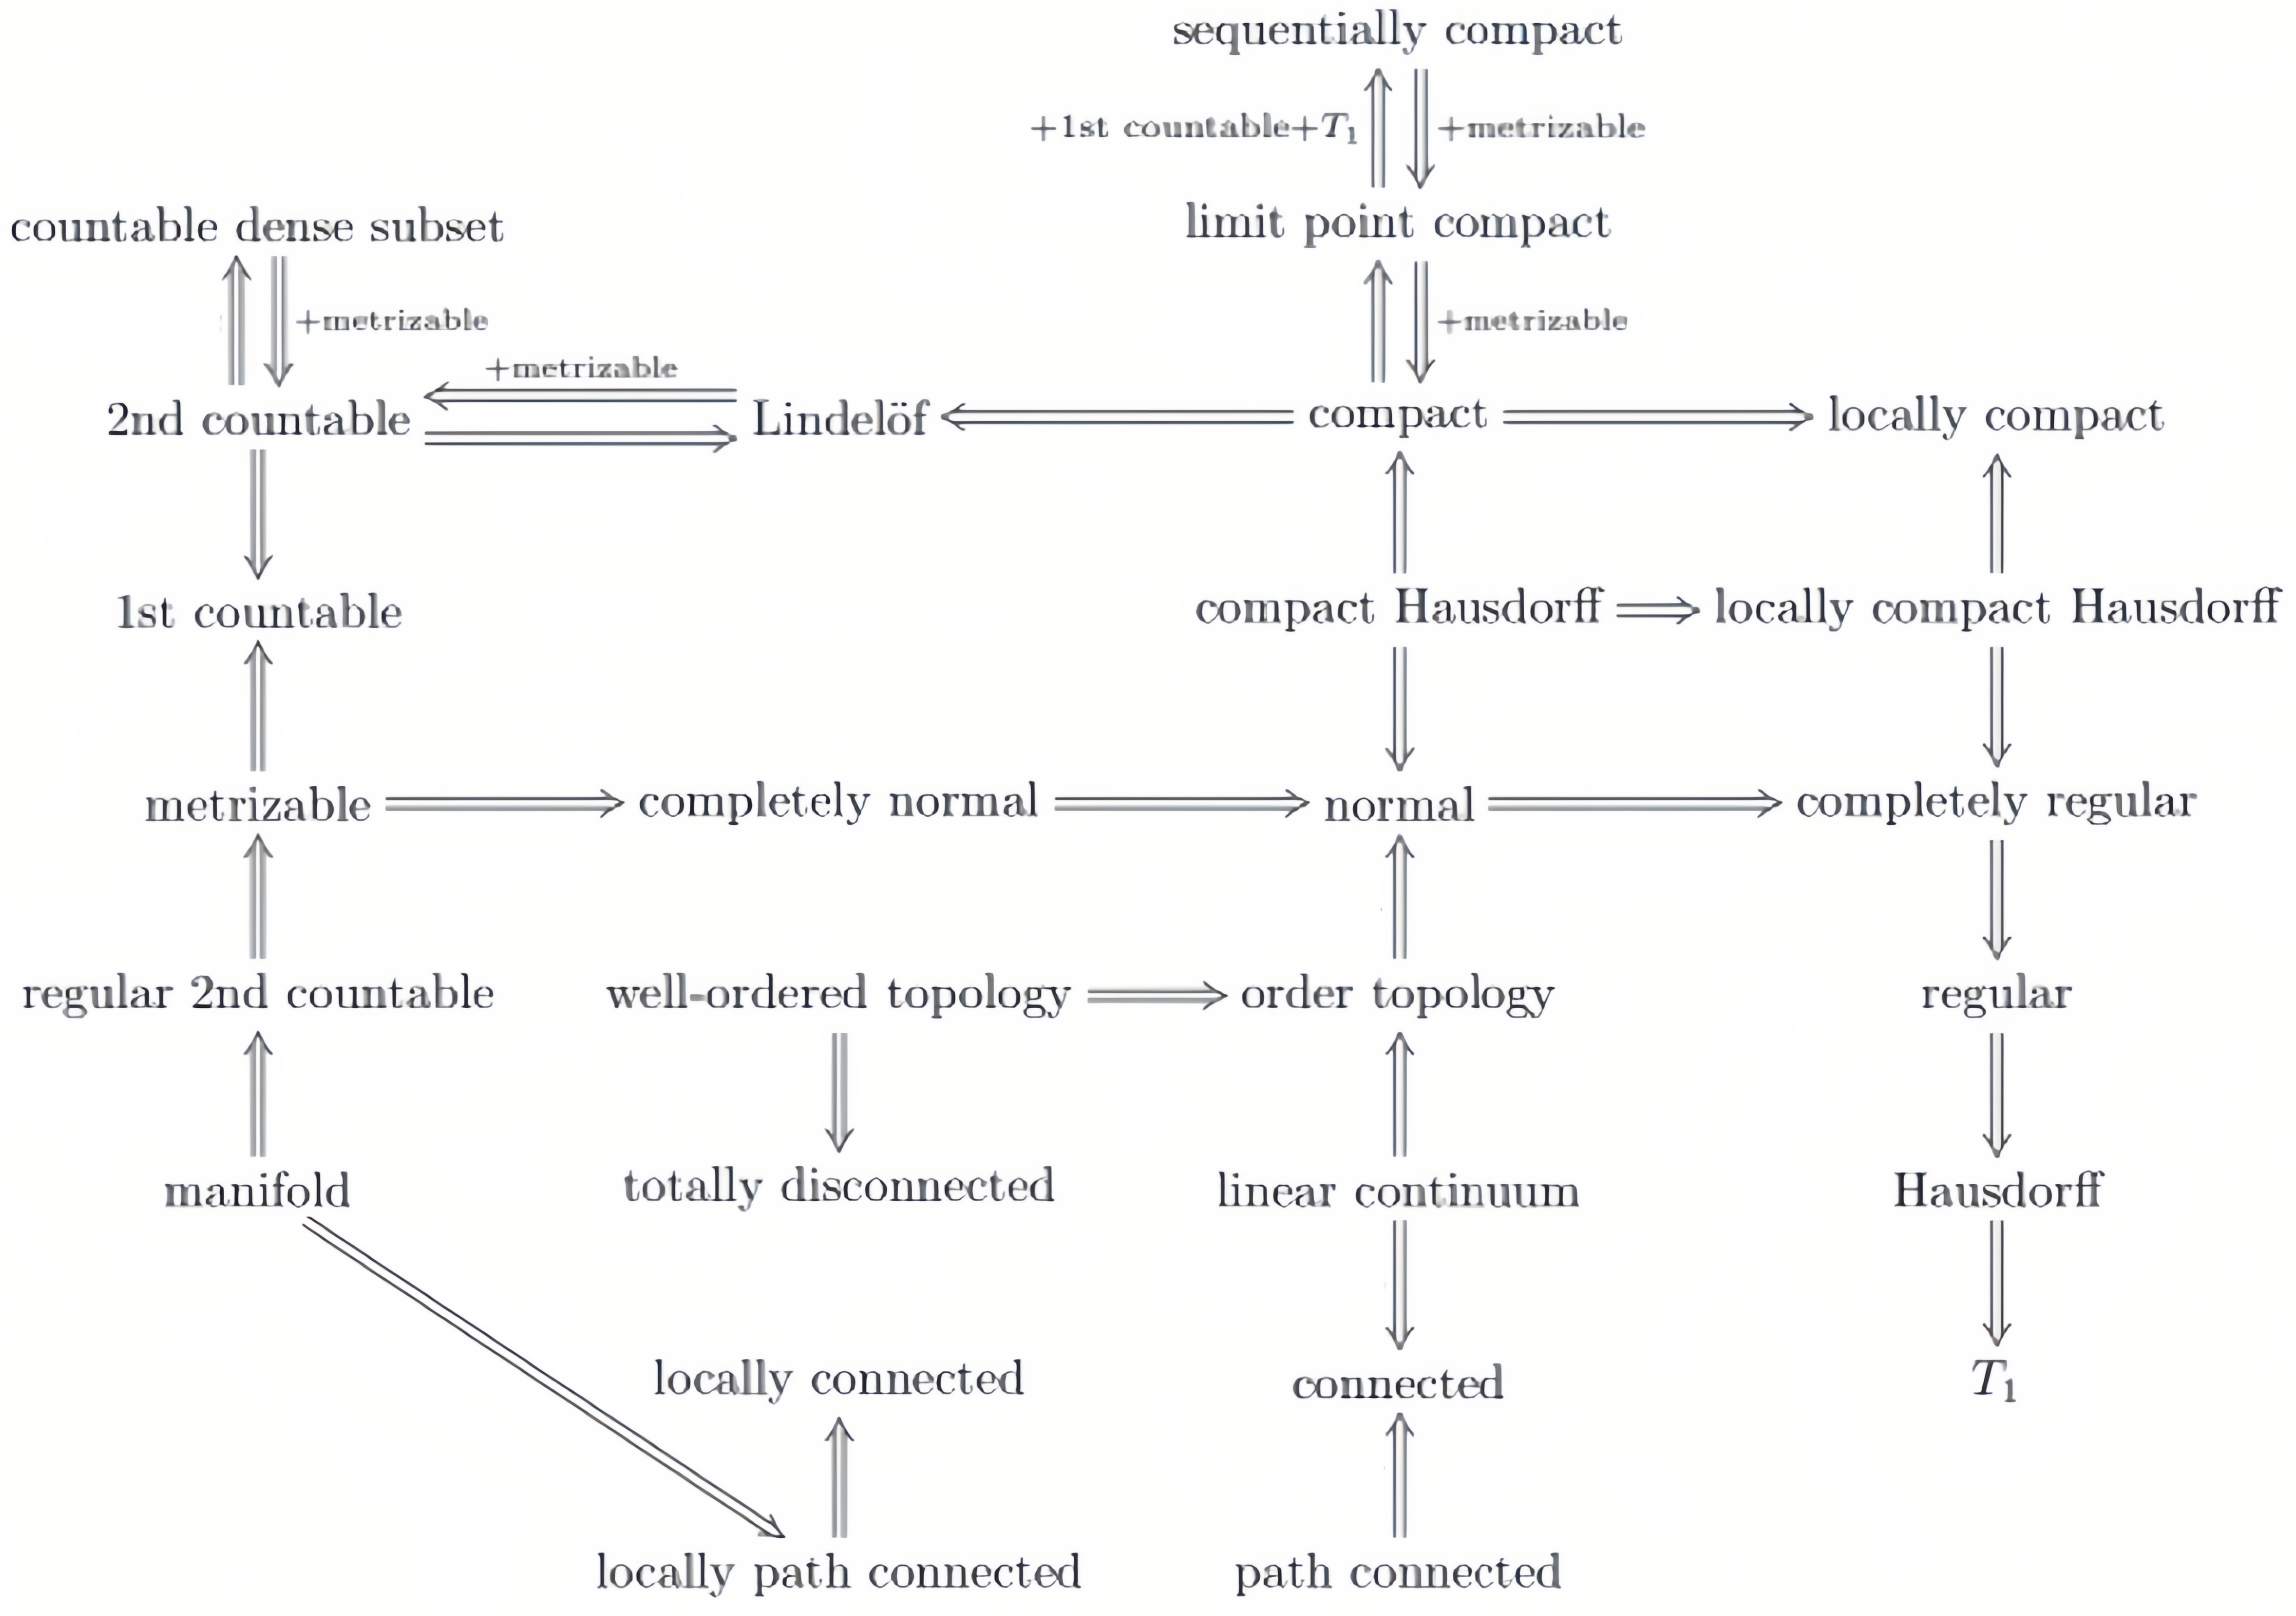
\includegraphics[width=1\textwidth]{制图2-vmake.png}
		\caption{Relations between topological spaces}
	\end{figure}
\end{abstract}% Vertical whitespace between the abstract and first section

%----------------------------------------------------------------------------------------
%	ESSAY BODY
%----------------------------------------------------------------------------------------
\section*{Introduction}
We have learned many different topological spaces that vary in structure, but share some relationships in terms of connectedness, compactness, and separateness. 
In this paper, we will give some definitions that were not mentioned in the class, and summarize the relations between some common topological spaces. 
Our work is shown in Figure 1.

\newpage

\section*{Additional Definitions}

\subsection*{1. Sets and maps}

\vskip 3pt
\textbf{Def 1.1 Linear order.} A linear order on the set $A$ is a relation $<\subset A \times A$ that is

\vskip 3pt
$\qquad$Comparable: If $a \not= b $ then $a < b$ or $b < a$ for all $a, b \in A$

\vskip 3pt
$\qquad$Nonreflexive: $a < a$ for no $a \in A$

\vskip 3pt
$\qquad$Transitive: $a < b$ and $b < c \implies a < c$ for all $a, b, c \in A$
%----------------------

\vskip 12pt
\textbf{Def 1.2 Dictionary order.} Let $(A, <)$ and $(B, <)$ be linearly ordered sets. 
The dictionary order on $A \times B$ is the linear order given by

\vskip -6pt
\begin{equation*}
	(a_1, b_1) < (a_2, b_2)  \Longleftrightarrow  (a_1 < a_2) \;or\; (a_1 = a_2 \;and\; b_1 < b_2)
\end{equation*}
\noindent
The restriction of a dictionary order to a product subspace is the dictionary order of the restricted
linear orders.
%----------------------

\vskip 12pt
\textbf{Def 1.3 Linear continuum.} An ordered set $(A, <)$ has the least upper bound property if any nonempty subset
of $A$ that has an upper bound has a least upper bound. 
If also $(x, y) \not= \emptyset$ for all $x < y$, then $(A, <)$ is a
linear continuum.
%----------------------

\vskip 12pt
\textbf{Def 1.4 Well-ordered sets.} A set $A$ with a linear order $<$ is well-ordered if any nonempty subset has a smallest
element.
%----------------------
\subsection*{2. Topological spaces and continuous maps}

\vskip 3pt
\textbf{Def 2.1 Order topology.} Let $(X, <)$ be a linearly ordered set containing at least two points.
The open rays in $X$ are the subsets
\begin{equation*}
	(-\infty, b) = \{x \in X \; | \; x < b\}\;,\; (a, +\infty) = \{x \in X \; | \; a < x\}
\end{equation*}
\noindent
of X. The order topology $T_<$ on the linearly ordered set $X$ is the topology generated by
all open rays. 
A linearly ordered space is a linearly ordered set with the order topology.
The open intervals in $X$ are the subsets of the form
\begin{equation*}
	(a, b) = (-\infty, b) \cap (a, +\infty) = \{x \in X \; | \; a < x < b\},\; a, b \in X, \;a < b.
\end{equation*}
%----------------------

\vskip 12pt
\textbf{Def 2.2 Separation axioms $T_0$, $T_1$, and $T_2$.}

\vskip 3pt
\textbf{$T_0$-space}: A topological space $X$ is a $T_0$-space (or a
Kolmogorov space) if for any two distinct points $x_1 \not= x_2$ in $X$ there exists an open set $U$ containing one
but not both points.

\vskip 3pt
\textbf{$T_1$-space}: A topological space is $T_1$-space if points are closed: For any two distinct points $x_1 \not= x_2$ in $X$ there
exists an open set $U$ such that $x_1 \in U$ and $x_2 \not\in U$.

\vskip 3pt
\textbf{$T_2$-space}: A topological space $X$ is a $T_2$-space (or a Hausdorff space) if there are enough open sets to separate
points: For any two distinct points $x_1 \not= x_2$ in $X$ there exist disjoint open sets, $U_1$ and $U_2$, such that
$x_1 \in U_1$ and $x_2 \in U_2$.
%----------------------

\vskip 12pt
\textbf{Def 2.3 Limit point compactness and sequential compactness.} A space $X$ is

\vskip 3pt
(1) limit point compact if any infinite subset of $X$ has a limit point.

\vskip 3pt
(2) sequentially compact if any sequence in $X$ has a convergent subsequence.
%----------------------

\vskip 12pt
\textbf{Def 2.4 Locally compact.}  A space $X$ is locally compact at the point $x \in X$ if $x$ lies in the interior of some
compact subset of $X$. 
A space is locally compact if it is locally compact at each of its points.
%----------------------

\subsection*{3. Regular and normal spaces}

\vskip 3pt
\textbf{Def 3.1 Lindelöf.} A topological space in which every open covering has a countable subcovering is called a Lindelöf Space.
%----------------------

\vskip 12pt
\textbf{Def 3.2 Completely regular.} A space $X$ is completely regular if points are closed in $X$ and for any closed
subset $C$ of $X$ and any point $x \not\in C$ there exists a continuous function $f : X \rightarrow [0, 1]$ such that $f (x) = 0$
and $f (C) = 1$.
%----------------------

\vskip 12pt
\textbf{Def 3.3 Completely normal.} A space $X$ is completely normal if every subspace of $X$ is normal, equivalent to the fact that for any two disjoint closed subsets of $X$ there exist disjoint open sets containing them.
%----------------------

\section*{Proof of Relations}

\subsection*{[Deduction 1]}
\vskip -10pt
\begin{equation}
	connected \overset{1}{\Longleftarrow} linear \; continuum \overset{2}{\Longrightarrow} order \; topology \overset{3}{\Longrightarrow} normal
\end{equation}

\vskip 10pt
\textbf{Proof 1.} [Lemma 1] Suppose that $X$ is a linear continuum. Then \cite{1}(2.118)
\begin{equation*}
	\{connected \; subsets \; of \; X\} = \{convex \; subsets \; of \; X\}
\end{equation*}

\vskip -5pt
Assume $X$ is a linear continuum. From [Lemma 1] we know that the the connected and the convex
subsets of $X$ are the same. In particular, the linear continuum $X$, certainly convex in itself, is connected
in the order topology. Let $C$ be a nonempty convex subset of $X$. We look at two cases:
\begin{itemize}
	\item \textbf{Case 1.} $C$ is neither bounded from above nor below. Let $x$ be any point of $X$. Since $x$ is neither a lower
	nor an upper bound for $C$ there exist $a, b \in C$ so that $a < x < b$. Then $x \in C$ by convexity.
	Thus $C = X$.

	\vskip 3pt
	\item\textbf{Case 2.} $C$ is bounded from above but not from below. Let $c = sup\; C$ be its least upper bound. Then
	$C \subset (-\infty, c]$. Let $x < c$ be any point. Since $x$ is neither a lower nor an upper bound for $C$
	there exist $a, b \in C$ so that $a < x < b$. Then $x \in C$ by convexity. Thus $(-\infty, c) \subset C \subset (-\infty, c]$
	and $C$ is either $(-\infty, c) \; or \; (-\infty, c]$.\

	\vskip 3pt
	\item \textbf{Case 3.} The arguments are similar for the other cases, since $X$ also has the greatest lower bound property
	\cite{2} (Ex 3.13).
\end{itemize}

\vskip 10pt
\textbf{Proof 2.} From Proof 1. we know that
\begin{equation*}
	X \; is \; a \; linear \; continuum \implies X \; is \; connected \; in \; the \; order \; topology 
\end{equation*}

\vskip 10pt
\textbf{Proof 3.} Linearly ordered spaces are normal.

\vskip 3pt
General proofs can be referred to \cite{3} (Problem 1.7.4). We shall only prove the special case that every well-ordered space is normal. 
\begin{itemize}
	\item \textbf{Step 1.} Let $X$ be a well-ordered set. In the order topology, sets of the form $(a, +\infty) = [a^+, +\infty ) =
	X - (-\infty, a]$, $(-\infty, b] = (-\infty, b+) = X - (b, +\infty)$ and $(a, b] = (a, +\infty) \cap (-\infty, b]$ are closed and open.

	\vskip 5pt
	\item \textbf{Step 2.} Let $A$ and $B$ be two disjoint closed subsets and
	let $a_0$ denote the smallest element of $X$. Suppose that neither $A$ nor $B$ contain $a_0$. For any point $a \in A$
	there exists a point $x_a < a$ such that $(x_a, a]$ is disjoint from $B$. Similarly, for any point $b \in B$ there
	exists a point $x_b < b$ such that $(x_b, b]$ is disjoint from $A$. The proof now proceeds as the proof for
	normality of $R_l$. Suppose next that $a_0 \in A \cup B$, say $a_0 \in A$. The one-point set ${a_0} = [a_0, a^+_0 )$ is open
	and closed (as $X$ is Hausdorff). By the above, we can find disjoint open sets $U , V$ such that $A-{a_0} \subset U$
	and $B \subset V$ . Then $A \subset U \cup {a_0}$ and $B \subset V - {a_0}$ where the open sets $U \cup {a_0}$ and $V - {a_0}$ are
	disjoint.
\end{itemize}
%----------------------

\vskip 10pt
\subsection*{[Deduction 2]}
\vskip -10pt
\begin{equation}
	well-ordered \; topology \overset{4}{\Longrightarrow} totally \; disconnected
\end{equation}

\vskip 10pt
\textbf{Proof 4.} A space is totally disconnected if its only connected subspaces are one-point
sets. Any well-ordered set $X$ containing at least two points is totally disconnected in the order topology.
For if $C \subset X$ contains $a < b$, then $a \not\in C \cap (a, b] \ni b$ is closed and open in $C$, since $(a, b]$ is closed and open
in $X$.
%----------------------

\vskip 10pt
\subsection*{[Deduction 3]}
\vskip -10pt
\begin{equation}
	compact \overset{5}{\Longrightarrow} limit \; point \; compact \overset{6\; (+1st\; countable + T_1)}{\Longrightarrow} sequentially \; compact 
\end{equation}

\vskip 10pt
\textbf{Proof 5.} [Lemma 2] Let $A$ be a subset of $X$ and $A'$ the set of limit points of $A$. Then $A \cup A' = A$
and $A \cap A' = \{a \in A \; | \; a \; is \; not \; an \; isolated \; point \; of \; A\}$ so that
$$
\begin{aligned}
	A \supset A' &\iff A \; is \; closed\\
	A \subset A' &\iff A \; has \; no \; isolated \; points\\
	A \cap A' = \emptyset&\iff A \; is \; discrete\\
	A' = \emptyset &\iff A \; is \; closed \; and \; discrete\\
\end{aligned}
$$
For any compact topological space $X$, a subset with no limit points is closed and
discrete [Lemma 2], hence finite (Any closed subspace of a compact space is compact).

\vskip 10pt
\textbf{Proof 6.} Let $X$ be a limit point compact space, 1st countable and $T_1$. Let $(x_n)$ be a sequence
in $X$. Consider the set $A = \{x_n \; | \; n \in Z_+\}$ of points in the sequence. 
\begin{itemize}
	\item \textbf{Case 1.} If $A$ is finite, there is a constant subsequence. 
	
	\vskip	5pt
	\item \textbf{Case 2.} If $A$ is infinite, $A$ has a limit point $x$ by hypothesis. As $X$ is 1st countable, there
	is a countable nested countable basis $U_1 \supset U_2 \supset \cdots$ at $x$ just as in the proof of \cite{1}(2.100). Since $x$ is a
	limit point, there is a sequence element $x_{n_1} \in U_1$ and we can find $n_1 < \cdots < n_k$ such that
	$x_{n_i} \in U_i$. Since $x$ is a limit point and $X$ is $T_1$, there are infinitely many points from $A$ in $U_{k+1}$. In
	particular, there is $n_{k+1} < n_k$ such that $x_{n_{k+1}}$ is in $U_{k+1}$. The subsequence $x_{n_k}$ converges to $x$.
\end{itemize}
%----------------------

\vskip 10pt
\subsection*{[Deduction 4]}
\vskip -10pt
\begin{equation}
	compact \overset{7\; (+metrizable)}{\Longleftarrow} limit \; point \; compact \overset{8\; (+metrizable)}{\Longleftarrow} sequentially \; compact 
\end{equation}

\vskip	10pt
\textbf{Proof 7. 8.} All three forms of compactness are equivalent for a metrizable space. 
It is well-known from our experience with metric spaces that 
\begin{equation*}
	X \; is \; sequentially \; compact \iff X \; is \; compact.
\end{equation*}
\noindent
Hence $X$ is sequentially compact and metrizable $\Rightarrow X$ compact, and due to Proof 5. the three forms of compactness are equivalent.
%----------------------

\vskip 10pt
\subsection*{[Deduction 5]}
\vskip -10pt
\begin{equation}
	countable \; dense \; subset \overset{9}{\Longleftarrow} 2nd \; countable \overset{10}{\Longrightarrow} Lindel\textit{ö}f
\end{equation}

\vskip 10pt
\textbf{Proof 9.} Suppose that $X$ is second countable and let $\mathcal{B}$ be a countable basis for the topology.
$X$ has a countable dense subset. Pick a point $b_B \in B$ in each basis set $B \in \mathcal{B}$. Then $\{b_B \; | \; B \in \mathcal{B}\}$ is
countable and dense.

\vskip 10pt
\textbf{Proof 10.} Let $\mathcal{U}$ be an open covering of $X$. For each basis set $B \in \mathcal{B}$ which is contained in some open
set from the collection $\mathcal{U}$, pick any $\mathrm{U}_B \in \mathcal{U}$ such that $B \subset \mathrm{U}_B$. Then the at most countable collection
$\{\mathrm{U}_B\}$ of these open sets from $\mathcal{U}$ is an open covering. Let $x$ be any point in $X$. Since $x$ is contained in a
member $\mathrm{U}$ of $\mathcal{U}$ and every open set is a union of basis sets, we have $x \in B \subset \mathrm{U}$ for some basis set $B \in \mathcal{B}$.
But then $x \in B \subset \mathrm{U}_B$.
%----------------------

\vskip 10pt
\subsection*{[Deduction 6]}
\vskip -10pt
\begin{equation}
	countable \; dense \; subset \overset{11\; (+metrizable)}{\Longrightarrow} 2nd \; countable \overset{12\; (+metrizable)}{\Longleftarrow} Lindel\textit{ö}f
\end{equation}

\vskip 10pt
\textbf{Proof 11.} Let $X$ be a metric space with a countable dense subset $A \subset X$. Then the collection $\{B(a, r) \;|\; a \in A, r \in Q_+\}$ of balls centered at
points in $A$ and with a rational radius is a countable basis for the topology. It suffices to show that for any open ball $B(x, \epsilon)$ in $X$ and any $y \in B(x, \epsilon)$ there are $a \in A$ and $r \in Q_+$
such that $y \in B(a, r) \subset B(x, \epsilon)$. Let $r$ be a positive rational number such that $2r + d(x, y) < \epsilon$
and let $a \in A \cap B(y, r)$. Then $y \in B(a, r)$, of course, and $B(a, r) \subset B(x, \epsilon)$ for if $d(a, z) < r$ then
$d(x, z) \leq d(x, y) + d(y, z) \leq d(x, y) + d(y, a) + d(a, z) < d(x, y) + 2r < \epsilon$.

\vskip 10pt
\textbf{Proof 12.} Let $X$ be a metric Lindelöf space. For each positive rational
number $r$, let $A_r$ be a countable subset of $X$ such that $X = \cup_{a\in A_r} B(a, r)$. Then $A = \cup_{r\in Q_+} A_r$ is a dense countable subset.
For any open ball $B(x, \epsilon)$ and any positive rational $r < \epsilon$ there is an
$a \in A_r$ such that $x \in B(a, r)$. Then $a \in B(x, r) \subset B(x, \epsilon)$.
%----------------------

\vskip 10pt
\subsection*{[Deduction 7]}
\vskip -10pt
\begin{equation}
	compact \; Hausdorff \overset{13}{\Longrightarrow} normal 
\end{equation}

\vskip 10pt
\textbf{Proof 13.} Let $X$ be a compact Hausdorff space. We claim that
$$\{compact \; subspaces \; of \; X\} \;=\; \{closed \; subspaces \; of \; X\}$$

Compact subspaces of Hausdorff spaces are closed, hence $\subset$, and closed subspaces of compact spaces are compact, hence $\supset$.
Let $A$ and $B$ be disjoint closed subsets of $X$, then $A$ and $B$ are compact as just shown.
Since any two disjoint compact subspaces of a Hausdorff space can be separated by disjoint open sets, there exist disjoint open sets $U , V$ such that $A \subset U$ and $B \subset V$ .
%----------------------

\vskip 10pt
\subsection*{[Deduction 8]}
\vskip -10pt
\begin{equation}
	completely \; regular \overset{14}{\Longleftarrow} locally \; compact \; Hausdorff
\end{equation}

\vskip 10pt
\textbf{Proof 14.} We will prove that locally compact Hausdorff spaces are open subspaces of compact spaces, and completely
regular spaces are subspaces of compact spaces.

\begin{itemize}
	\item \textbf{Step 1.} For a Hausdorff space $X$,
	$$X \; is \; locally \; compact \iff X \; is \; homeomorphic \; to \; an \; open \; subset \; of \; a \; compact \; space$$
	The locally compact Hausdorff space $X$ is homeomorphic to the open subspace $\omega X - \{\omega\}$ of the compact Hausdorff space $\omega X$, where $\omega X = X \cup \{\omega\}$ denote the union of $X$ with a set consisting of a single point $\omega$.
	Hence locally compact Hausdorff spaces are open subspaces of compact spaces.

	\vskip 5pt
	\item \textbf{Step 2.} For a topological space $X$,
	$$X \; is \; completely \; regular \iff X \cong  a \; subspace \; of \; a \; compact \; Hausdorff \; space$$
	If $X$ is completely regular then the set $C(X)$ of continuous maps $X \rightarrow [0, 1]$ separates points and closed sets. The evaluation map
	$$\Delta: X \rightarrow \textstyle{\prod_{j\in C(X)}}[0,1], \;\pi_j (\Delta(x)) = j(x),\; j \in C(X),\; x \in X$$
is therefore an embedding. By the Tychonoff theorem\cite{1}(2.149), $[0, 1]^J$ is compact Hausdorff. A compact Hausdorff space is normal, hence completely regular and subspaces of completely regular spaces are completely regular.
\end{itemize}
%----------------------

\vskip 10pt
\subsection*{[Deduction 9]}
\vskip -10pt
\begin{equation}
	manifold \overset{15}{\Longrightarrow} regular \; 2nd \; countable \overset{16}{\Longrightarrow} metrizable
\end{equation}

\vskip 10pt
\textbf{Proof 15.} According to the definition of manifolds, every point has a neighbourhood that is homeomorphic to some $R^n$.
So this means (as $R^n$ is locally compact) that every manifold is locally compact
and a locally compact Hausdorff space is (completely) regular.

\vskip 10pt
\textbf{Proof 16.} [Urysohn metrization theorem] The following conditions are equivalent for a second
countable space $X$: (1) $X$ is regular; (2) $X$ is normal; (3) $X$ is homeomorphic to a subspace of $[0, 1]^\omega$, where the Hilbert cube $[0, 1]^\omega$ is a universal second countable metrizable (or normal or regular) space; (4) $X$ is metrizable.\cite{1}(3.27)

%----------------------

\section*{Summary}

In [Deduction 1-9], we have proved that
$$
\begin{aligned}
&	connected \overset{1}{\Longleftarrow} linear \; continuum \overset{2}{\Longrightarrow} order \; topology \overset{3}{\Longrightarrow} normal
\\
&	well-ordered \; topology \overset{4}{\Longrightarrow} totally \; disconnected
\\
&	compact \overset{5}{\Longrightarrow} limit \; point \; compact \overset{6\; (+1st\; countable + T_1)}{\Longrightarrow} sequentially \; compact 
\\
&	compact \overset{7\; (+metrizable)}{\Longleftarrow} limit \; point \; compact \overset{8\; (+metrizable)}{\Longleftarrow} sequentially \; compact 
\\
&	countable \; dense \; subset \overset{9}{\Longleftarrow} 2nd \; countable \overset{10}{\Longrightarrow} Lindel\textit{ö}f
\\
&	countable \; dense \; subset \overset{11\; (+metrizable)}{\Longrightarrow} 2nd \; countable \overset{12\; (+metrizable)}{\Longleftarrow} Lindel\textit{ö}f
\\
&	compact \; Hausdorff \overset{13}{\Longrightarrow} normal 
\\
&	completely \; regular \overset{14}{\Longleftarrow} locally \; compact \; Hausdorff
\\
&	manifold \overset{15}{\Longrightarrow} regular \; 2nd \; countable \overset{16}{\Longrightarrow} metrizable.\\
\end{aligned}
$$

\vskip 10pt
The following deductions can be easily proved by the definitions.
$$
\begin{aligned}
&well-ordered \; topology \overset{~}{\Longrightarrow} ordered \; topology\\
&Lindel\textit{ö}f \overset{~}{\Longleftarrow} compact \overset{~}{\Longrightarrow} locally \; compact \overset{~}{\Longrightarrow} locally \; compact\\
&compact \overset{~}{\Longleftarrow} compact \; Hausdorff \overset{~}{\Longrightarrow} locally \; compact \; Hausdorff \\
&locally \; compact \; Hausdorff \overset{~}{\Longrightarrow} locally \; compact\\
&completely \; normal \overset{~}{\Longrightarrow} normal \overset{~}{\Longrightarrow} completely \; regular \overset{~}{\Longrightarrow} regular\\
&rugular \overset{~}{\Longrightarrow} Hausdorff \overset{~}{\Longrightarrow} T_1\\
&2nd \; countable \overset{~}{\Longrightarrow} 1st \; countable \overset{~}{\Longleftarrow} metrizable\\
&manifold \overset{~}{\Longrightarrow} locally \; path \; connected \overset{~}{\Longrightarrow} locally \; connected\\
\end{aligned}
$$

\vskip 10pt
Above all, we have proved the relations between topological spaces shown in Figure 1.
%----------------------------------------------------------------------------------------

\vskip 25pt
\textit{Thanks to my General Topology teacher, Youlin Li, for his guidence and the authors of \cite{1}\cite{2}\cite{3} for their wonderful ideas.}
%----------------------------------------------------------------------------------------
%	BIBLIOGRAPHY
%----------------------------------------------------------------------------------------

%\bibliographystyle{unsrt}
\vskip 30pt
\bibliography{sample.bib}

%----------------------------------------------------------------------------------------
\end{document}
